\documentclass[border=2pt]{standalone}
\usepackage{pgfplots}
\usetikzlibrary{arrows.meta}
\definecolor{blogred}{HTML}{ff6868}
\begin{document}
    \resizebox{10cm}{!} {
        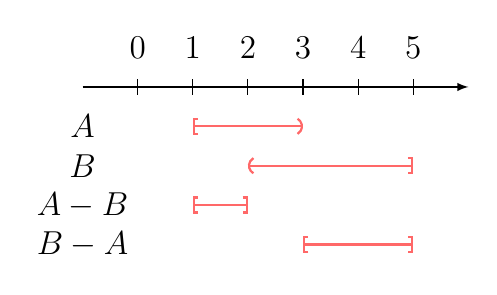
\begin{tikzpicture} [
            xscale = 0.7,
            yscale = -1
        ]
            \tikzset{basestyle/.style = {thick, blogred}}
            \tikzset{crange/.style    = {basestyle, Bracket-Bracket}}
            \tikzset{orange/.style    = {basestyle, Parenthesis-Parenthesis}}
            \tikzset{lorange/.style   = {basestyle, Parenthesis-Bracket}}
            \tikzset{rorange/.style   = {basestyle, Bracket-Parenthesis}}

            % x-axis specification
            \draw [-latex] (-1,0) -- (6,0);
            \foreach \x in {0,1,...,5} {
                \draw (\x, 0.1) -- (\x,-0.1);
                \draw (\x,-0.5) node {\large $\x$};
            }

            \draw (-1,0.5) node {\large $A$};
            \draw [rorange] (1,0.5) -- (3,0.5);

            \draw (-1,1.0) node {\large $B$};
            \draw [lorange] (2,1.0) -- (5,1.0);

            \draw (-1,1.5) node {\large $A - B$};
            \draw [crange] (1,1.5) -- (2,1.5);

            \draw (-1,2.0) node {\large $B - A$};
            \draw [crange] (3,2.0) -- (5,2.0);
        \end{tikzpicture}
    }
\end{document}
